\chapter{DETERMINANTES}

El estudio de los determinantes adquiere relevancia primordial al abordar la noción de invertibilidad de las matrices. Su presencia y magnitud se convierten en criterios decisivos para determinar si una matriz posee una inversa, un concepto esencial en la resolución de sistemas lineales y en el análisis de transformaciones lineales.\infoBulle{Se debe mencionar que durante un tiempo los determinantes jugaron un papel fundamental en el estudio del álgebra lineal; ahora, sin embargo, tienen una importancia mucho menor. Veremos, de hecho, que virtualmente nuestra única utilización de los determinantes será en el cálculo de los “eigenvalores”.}

Además, la conexión intrínseca entre los determinantes y la geometría añade otra dimensión de fascinación. No se limitan meramente a manipulaciones algebraicas; los determinantes encuentran aplicación directa en la determinación de áreas y volúmenes en espacios euclidianos, estableciendo un puente conceptual entre el álgebra y la geometría. La relación entre los determinantes y la geometría amplía nuestro entendimiento matemático y resalta la belleza de su interrelación. Explorar cómo se entrelazan con la estructura geométrica de los espacios vectoriales nos permite apreciar la profundidad y la elegancia de las matemáticas en su conjunto.

\section{Determinantes por expansión de cofactores}

\begin{definicion}{}{}
    Consideremos una matriz de tamaño $2 \times 2$
    $$A = \begin{bmatrix}
        a & b \\
        c & d
    \end{bmatrix}.$$
    Definimos el determinante de dicha matriz, escribiendo
    \begin{equation}
        \det(A) = ad - bc \quad \text{ o } \quad \begin{vmatrix}
            a & b \\
            c & d
        \end{vmatrix} = ad - bc. \label{defdeterminante}
    \end{equation}
\end{definicion}

A continuación, demostraremos un teorema que relaciona el determinante y la inversa de una matriz.\infoBulle{Es importante considerar que $\det(A)$ es un número, mientras que $A$ es una matriz.}

\newpage

\begin{theorem}{}{USJSJSSSJKSIIS}
    Sea $A$ una matriz de tamaño $2 \times 2$.
    \begin{enumerate}[label=\roman*), topsep=6pt, itemsep=0pt]
        \item $A$ es invertible si y solo si $\det(A) \neq 0$.
        \item Si $\det(A) \neq 0$, entonces
        \begin{equation}
            A^{-1} = \frac{1}{\det(A)} \begin{bmatrix*}[r]
                d & -b \\
                -c & a
            \end{bmatrix*}. \label{determinante-inversa}
        \end{equation}
    \end{enumerate}

    \tcblower
    \demostracion
    \begin{enumerate}[label=\roman*), topsep=6pt, itemsep=0pt]
        \item Supongamos que $A$ es invertible. Entonces existe $A^{-1}$ tal que $AA^{-1} = I$. Si $\det(A) = 0$, entonces $ad - bc = 0$. Consideremos el sistema homogéneo asociado $A\mathbb{x} = \mathbb{0}$,
        \begin{align*}
            ax_1 + bx_2 & = 0 \\
            cx_1 + dx_2 & = 0
        \end{align*}
        Como $ad - bc = 0$, las filas de $A$ son linealmente dependientes, y el sistema tiene soluciones no triviales. Sin embargo, si $A$ es invertible, el único vector $\mathbb{x}$ que satisface $A\mathbb{x} = \mathbb{0}$ es $\mathbb{x} = \mathbb{0}$. Esta contradicción implica que $\det(A) \neq 0$. Ahora bien, supongamos que $\det(A) \neq 0$ y sea
        \begin{equation}
            B = \frac{1}{\det(A)} \begin{bmatrix*}[r]
                d & -b \\
                -c & a
            \end{bmatrix*}. \label{JAJAJIAOQOSIHWTEEYYWYQYWCXZZZ}
        \end{equation}
        Entonces,
        \begin{align*}
            BA & = \frac{1}{\det(A)} \begin{bmatrix*}[r]
                d & -b \\
                -c & a
            \end{bmatrix*} \begin{bmatrix}
                a & b \\
                c & d
            \end{bmatrix} \\
            & = \frac{1}{ad - bc} \begin{bmatrix}
                da - bc & 0 \\
                0 & -cb + ad
            \end{bmatrix} \\
            & = \begin{bmatrix}
                1 & 0 \\
                0 & 1
            \end{bmatrix}
        \end{align*}
        De manera similar, $AB = I$. De esta manera, $AB = BA = I$, por lo que $A$ es invertible y $B = A^{-1}$.
        \item Del inciso anterior, si $\det(A) \neq 0$, entonces $A$ es invertible, y la matriz $B$ definida en \eqref{JAJAJIAOQOSIHWTEEYYWYQYWCXZZZ}, satisface $AB = BA = I$. Por tanto,
        $$A^{-1} = \frac{1}{\det(A)} \begin{bmatrix*}[r]
            d & -b \\
            -c & a
        \end{bmatrix*}.$$
    \end{enumerate}
\end{theorem}

Uno de nuestros principales objetivos en este capítulo es obtener un análogo de la fórmula \eqref{determinante-inversa} que sea aplicable a matrices cuadradas de todos los órdenes. Para este propósito, nos resultará conveniente usar entradas con subíndices al escribir matrices o determinantes. Así, si denotamos una matriz $2 \times 2$ como
$$A = \begin{bmatrix}
    a_{11} & a_{12} \\
    a_{21} & a_{22}
\end{bmatrix}$$
entonces las dos ecuaciones en \eqref{defdeterminante} toman la forma
\begin{equation}
    \det(A) = \begin{vmatrix}
        a_{11} & a_{12} \\
        a_{21} & a_{22}
    \end{vmatrix} = a_{11}a_{22} - a_{12}a_{21}. \label{eq:determinantesubi}
\end{equation}
En situaciones donde no sea conveniente asignar un nombre a la matriz, podemos expresar esta fórmula como
\begin{equation}
    \det\left(\begin{bmatrix}
        a_{11} & a_{12} \\
        a_{21} & a_{22}
    \end{bmatrix}\right) = a_{11}a_{22} - a_{12}a_{21}. \label{JAJAJIQIQIOPPQOPQPPPPPQO}
\end{equation}
\newpage\noindent
Existen varios métodos para definir determinantes de matrices cuadradas de orden superior. En este texto, el determinante de una matriz de $n \times n$ se definirá de manera inductiva. En otras palabras, se usará lo que se sabe sobre un determinante de $2 \times 2$ para definir un determinante de $3 \times 3$, que a su vez se usará para definir un determinante de $4 \times 4$, y así sucesivamente. Para iniciar el proceso, definamos el determinante de una matriz $1 \times 1$ como
$$\det\left([a_{11}]\right) = a_{11}$$
de donde se deduce que la fórmula \eqref{JAJAJIQIQIOPPQOPQPPPPPQO} puede expresarse como
$$\det\left(\begin{bmatrix}
    a_{11} & a_{12} \\
    a_{21} & a_{22}
\end{bmatrix}\right) = \det\left([a_{11}]\right) \det\left([a_{22}]\right) - \det\left([a_{12}]\right) \det\left([a_{21}]\right).$$

Ahora que hemos establecido un punto de partida, podemos definir determinantes de matrices $3 \times 3$ en términos de determinantes de matrices $2 \times 2$, luego determinantes de matrices $4 \times 4$ en términos de determinantes de matrices $3 \times 3$, y así sucesivamente. La siguiente terminología y notación ayudarán a hacer este proceso inductivo más eficiente.

\begin{definicion}{}{}
    Si $A$ es una matriz cuadrada, entonces el \emph{menor de la entrada $a_{ij}$} se denota por $M_{ij}$ y se define como el determinante de la submatriz que permanece después de que la $i$-ésima fila y la $j$-ésima columna se eliminen de $A$. El número $(-1)^{i+j} M_{ij}$ se denota por $C_{ij}$ y se llama \emph{cofactor de la entrada $a_{ij}$.}
\end{definicion}

\begin{examplebox}{}{}
    Consideremos la matriz
    \begin{matrizn}
        \makecell{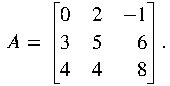
\includegraphics[page=1]{Externalizacion/C3/MatricesC3.pdf}}
    \end{matrizn}
    El menor de la entrada $a_{11}$ es
    \begin{matrizn}
        \makecell{\includegraphics[page=2]{Externalizacion/C3/MatricesC3.pdf}}
    \end{matrizn}
    El cofactor de $a_{11}$ es
    $$C_{11} = (-1)^{1 + 1} M_{11} = M_{11} = 16.$$
    Del mismo modo, el menor de la entrada $a_{32}$ es
    \begin{matrizn}
        \makecell{\includegraphics[page=3]{Externalizacion/C3/MatricesC3.pdf}}
    \end{matrizn}
    El cofactor de $a_{32}$ es
    $$C_{32} = (-1)^{3 + 2} M_{32} = -M_{32} = -26.$$
\end{examplebox}
\infoBulle{Hemos seguido la convención estándar de utilizar letras mayúsculas para denotar menores y cofactores aunque sean números, no matrices.}

Notemos que un menor $M_{ij}$ y su cofactor correspondiente $C_{ij}$ son iguales o negativos el uno del otro y que la relación de signo $(-1)^{i+j}$ es $+1$ o $-1$ de acuerdo con el patrón en la “matriz de tablero de ajedrez”
\begin{matrizn}
    \makecell{\includegraphics[page=4]{Externalizacion/C3/MatricesC3.pdf}}
\end{matrizn}
Por ejemplo,
$$C_{11} = M_{11}, \quad C_{21} = -M_{21}, \quad C_{22} = M_{22}$$
\newpage\noindent
y así sucesivamente. Así, nunca es realmente necesario calcular $(-1)^{i+j}$ para obtener $C_{ij}$. Se puede simplemente calcular el menor $M_{ij}$ y luego ajustar el signo de acuerdo con el patrón del tablero de ajedrez.

\begin{examplebox}{}{}
    El patrón del tablero de ajedrez para una matriz $A$ de tamaño $2 \times 2$ es
    $$\begin{bmatrix}
        + & - \\
        - & +
    \end{bmatrix}$$
    De esta manera: $C_{11} = M_{11} = a_{22}$, $C_{12} = -M_{12} = -a_{21}$, $C_{21} = -M_{21} = -a_{12}$, $C_{22} = M_{22} = a_{11}$. Dejamos al lector usar la fórmula \eqref{eq:determinantesubi} para verificar que $\det(A)$ puede expresarse en términos de cofactores de las siguientes cuatro maneras:
    \begin{equation}
        \begin{aligned}
            \det(A) & = \begin{vmatrix} a_{11} & a_{12} \\ a_{21} & a_{22} \end{vmatrix} \\
            & = a_{11} C_{11} + a_{12} C_{12} \\
            & = a_{21} C_{21} + a_{22} C_{22} \\
            & = a_{11} C_{11} + a_{21} C_{21} \\
            & = a_{12} C_{12} + a_{22} C_{22}
        \end{aligned} \label{eq:determinanpcofactores}
    \end{equation}
    Cada una de las cuatro ecuaciones se llama una \emph{expansión por cofactores} de $\det(A)$. En cada expansión por cofactores, las entradas y los cofactores provienen todos de la misma fila o de la misma columna de $A$. Por ejemplo, en la primera ecuación las entradas y cofactores provienen todos de la primera fila de $A$, en la segunda provienen todos de la segunda fila de $A$, en la tercera provienen todos de la primera columna de $A$, y en la cuarta provienen todos de la segunda columna de $A$.
\end{examplebox}

La fórmula \eqref{eq:determinanpcofactores} es un caso especial del siguiente resultado general, que presentaremos sin demostración.

\begin{theorem}{}{determinanteindecolfila}
    Si $A$ es una matriz $n \times n$, entonces independientemente de qué fila o columna de $A$ se elija, el número obtenido al multiplicar las entradas de esa fila o columna por los cofactores correspondientes y sumar los productos resultantes es el mismo.
\end{theorem}

Este resultado nos permite establecer la siguiente definición.

\begin{definicion}{}{}
    Si $A$ es una matriz $n \times n$, entonces el número obtenido al multiplicar las entradas de cualquier fila o columna de $A$ por los cofactores correspondientes y sumar los productos resultantes se llama \emph{determinante de $A$}, y las sumas en sí mismas se denominan \emph{expansiones por cofactores de $A$}. Es decir, el determinante se puede obtener mediante expansión por cofactores a lo largo de la $j$-ésima columna
    \begin{equation}
        \det(A) = a_{1j} C_{1j} + a_{2j} C_{2j} + \cdots + a_{nj} C_{nj} \label{eq:determinantecofcolumna}
    \end{equation}
    o bien, mediante expansión por cofactores a lo largo de la $i$-ésima fila
    \begin{equation}
        \det(A) = a_{i1} C_{i1} + a_{i2} C_{i2} + \cdots + a_{in} C_{in}. \label{eq:determinantecoffila}
    \end{equation}
\end{definicion}

\begin{examplebox}{}{primerdetcof}
    Encuentra el determinante de la matriz
    \begin{matrizn}
        \makecell{\includegraphics[page=5]{Externalizacion/C3/MatricesC3.pdf}}
    \end{matrizn}
    por expansión de cofactores a lo largo de la primera fila.

    \tcblower
    \solucion
    \begin{align*}
        \det(A) & = 3 \begin{vmatrix*}[r]
            -4 & 3 \\
            4 & -2
        \end{vmatrix*} - 1 \begin{vmatrix*}[r]
            -2 & 3 \\
            5 & -2
        \end{vmatrix*} + 0 \begin{vmatrix*}[r]
            -2 & -4 \\
            5 & 4
        \end{vmatrix*} \\
        & = 3(-4) - (1)(-11) + 0 = -1
    \end{align*}
\end{examplebox}

\newpage

\begin{examplebox}{}{segundodetcof}
    Sea $A$ la matriz del ejemplo \ref{examplebox:primerdetcof}, evalúe $\det(A)$ mediante la expansión de cofactores a lo largo de la primera columna de $A$.

    \tcblower
    \solucion
    \begin{align*}
        \det(A) & = 3 \begin{vmatrix*}[r]
            -4 & 3 \\
            4 & -2
        \end{vmatrix*} - (-2) \begin{vmatrix*}[r]
            1 & 0 \\
            4 & -2
        \end{vmatrix*} + 5 \begin{vmatrix*}[r]
            1 & 0 \\
            -4 & 3
        \end{vmatrix*} \\
        & = 3(-4) - (-2)(-2) + 5(3) = -1
    \end{align*}
    Esto concuerda con el resultado obtenido en el ejemplo \ref{examplebox:primerdetcof}.
\end{examplebox}

Tenga en cuenta que en el ejemplo \ref{examplebox:segundodetcof} tuvimos que calcular tres cofactores, mientras que en el ejemplo \ref{examplebox:primerdetcof} solo se necesitaban dos porque el tercero se multiplicó por cero. Como regla general, la mejor estrategia para la expansión de cofactores es expandirse a lo largo de una fila o columna con más ceros.

\begin{examplebox}{}{}
    Si $A$ es una matriz de $4 \times 4$ dada por
    \begin{matrizn}
        \makecell{\includegraphics[page=6]{Externalizacion/C3/MatricesC3.pdf}}
    \end{matrizn}
    Entonces para encontrar $\det(A)$ será más fácil usar la expansión de cofactores a lo largo de la segunda columna, ya que tiene la mayor cantidad de ceros:
    \begin{matrizn}
        \makecell{\includegraphics[page=7]{Externalizacion/C3/MatricesC3.pdf}}
    \end{matrizn}
    Para el determinante $3 \times 3$, será más fácil utilizar la expansión del cofactor a lo largo de su segunda columna, ya que tiene la mayor cantidad de ceros:
    $$\det(A) = -2 \cdot \begin{vmatrix*}[r]
        1 & -1 \\
        2 & 1
    \end{vmatrix*} = -2(1 + 2) = -6.$$
\end{examplebox}

\begin{examplebox}{}{}
    El siguiente cálculo muestra que el determinante de una matriz triangular inferior de $4 \times 4$ es el producto de sus elementos en la diagonal principal. Cada parte del cálculo utiliza una expansión de cofactores a lo largo de la primera fila.
    \begin{matrizn}
        \makecell{\includegraphics[page=8]{Externalizacion/C3/MatricesC3.pdf}}
    \end{matrizn}
\end{examplebox}

El método visto en el ejemplo anterior se puede generalizar fácilmente para demostrar el siguiente teorema.

\begin{theorem}{}{determinantetriangular}
    Si $A$ es una matriz $n \times n$ triangular superior o triangular inferior, entonces
    $$\det(A) = a_{11} a_{22} \cdots a_{nn}.$$
    Es decir, el determinante de una matriz triangular superior o inferior es igual al producto de sus componentes en la diagonal.

    \newpage
    \demostracion La parte triangular inferior del teorema se deja como ejercicio al lector (se puede deducir del ejemplo anterior). Se demostrará la parte triangular superior por inducción matemática sobre $n$, empezando por $n = 2$. Si $A$ es una matriz triangular superior de $2 \times 2$, entonces
    $$A = \begin{bmatrix}
        a_{11} & a_{12} \\
        0 & a_{22}
    \end{bmatrix}$$
    y $\det(A) = a_{11} a_{22} - a_{12} \cdot 0 = a_{11}a_{22}$ de manera que el teorema se cumple para $n = 2$. Se supondrá que se cumple para $k = n-1$ y se demostrará para $k = n$. El determinante de una matriz triangular superior de $n \times n$ es
    \begin{matrizn}
        \makecell{\includegraphics[page=9]{Externalizacion/C3/MatricesC3.pdf}}
    \end{matrizn}
    Cada uno de estos determinantes es el determinante de una matriz triangular superior de $(n - 1) \times (n - 1)$ que, de acuerdo con la hipótesis de inducción, es igual al producto de las componentes en la diagonal. Todas las matrices, excepto la primera, tienen una columna de ceros, por lo que por lo menos una de sus componentes diagonales es cero. De este modo, todos los determinantes, excepto el primero, son cero. Por último,
    \begin{matrizn}
        \makecell{\includegraphics[page=10]{Externalizacion/C3/MatricesC3.pdf}}
    \end{matrizn}
    lo que prueba que el teorema se cumple para matrices de $n \times n$.
\end{theorem}

Los determinantes de matrices $2 \times 2$ y $3 \times 3$ pueden evaluarse muy eficientemente usando el siguiente patrón:\infoBulle{La técnica de flechas para una matriz de $3 \times 3$ se le conoce como \emph{regla de Sarrus}. Esta solo funciona con determinantes de matrices de $3 \times 3$. No funciona con matrices de tamaño $4 \times 4$ o superior.}
\begin{matrizn}
    \makecell{\includegraphics[page=11]{Externalizacion/C3/MatricesC3.pdf}}
\end{matrizn}
En el caso $2 \times 2$, el determinante puede calcularse formando el producto de las entradas en la flecha hacia abajo y restando el producto de las entradas en la flecha hacia arriba. En el caso $3 \times 3$, primero copiamos las dos primeras columnas como se muestra en la figura, después de lo cual podemos calcular el determinante sumando los productos de las entradas en las flechas hacia abajo y restando los productos de las flechas hacia arriba. Estos procedimientos nos dan como resultado
$$\begin{vmatrix}
    a_{11} & a_{12} \\
    a_{21} & a_{22}
\end{vmatrix} = a_{11}a_{22} - a_{12}a_{21}$$
y
\begin{matrizn}
    \makecell{\includegraphics[page=12]{Externalizacion/C3/MatricesC3.pdf}}
\end{matrizn}
\newpage\noindent
lo que concuerda con las expansiones por cofactores a lo largo de la primera fila.

\begin{examplebox}{}{}
    Aplicando la regla de Sarrus a la matriz del ejemplo \ref{examplebox:primerdetcof}, obtenemos que:
    $$\makecell{\includegraphics[page=13]{Externalizacion/C3/MatricesC3.pdf}}$$
    lo que concuerda con el resultado obtenido en el ejemplo \ref{examplebox:primerdetcof}.
\end{examplebox}

\section{Evaluación de determinantes por reducción de filas}

En esta sección mostraremos cómo evaluar un determinante reduciendo la matriz asociada a forma escalonada por filas. En general, este método requiere menos cálculos que la expansión por cofactores y, por lo tanto, es el método de elección para matrices grandes.

Comenzamos con un teorema fundamental que nos llevará a un procedimiento eficiente para evaluar el determinante de una matriz cuadrada de cualquier tamaño.

\begin{theorem}{}{determinantefilcol0}
    Si $A$ tiene una fila de ceros o una columna de ceros, entonces $\det(A) = 0$.

    \tcblower
    \demostracion Dado que el determinante de $A$ puede encontrarse mediante una expansión por cofactores a lo largo de cualquier fila o columna, podemos usar la fila o columna de ceros. Si denotamos por $C_1, C_2, \dots, C_n$ a los cofactores de $A$ a lo largo de esa fila o columna, entonces se sigue de la fórmula \eqref{eq:determinantecofcolumna} o \eqref{eq:determinantecoffila} que
    $$\det(A) = 0 \cdot C_1 + 0 \cdot C_2 + \cdots + 0 \cdot C_n = 0.$$
\end{theorem}

El siguiente teorema útil relaciona el determinante de una matriz con el determinante de su transpuesta.

\begin{theorem}{}{}
    Sea $A$ una matriz cuadrada. Entonces $\det(A) = \det\left(A^T\right)$.

    \tcblower
    \demostracion Dado que trasponer una matriz cambia sus columnas por filas y sus filas por columnas, la expansión por cofactores de $A$ a lo largo de cualquier fila es la misma que la expansión por cofactores de $A^T$ a lo largo de la columna correspondiente. Así, ambos tienen el mismo determinante.
\end{theorem}

El siguiente teorema muestra cómo una operación elemental en el renglón de una matriz cuadrada afecta el valor de su determinante, proporcionando así una herramienta fundamental para el cálculo eficiente del determinante.

\begin{theorem}{}{determinanteconopelementales}
    Sea $A$ una matriz $n \times n$.
    \begin{enumerate}[label=\alph*), topsep=6pt, itemsep=0pt]
        \item Si $B$ es la matriz que resulta cuando un solo renglón o una sola columna de $A$ se multiplica por un escalar $k$, entonces $\det(B) = k \det(A)$.
        \item Si $B$ es la matriz que resulta cuando dos renglones o dos columnas de $A$ se intercambian, entonces $\det(B) = -\det(A)$.
        \item Si $B$ es la matriz que resulta cuando se agrega un múltiplo de un renglón de $A$ a otro, o cuando se agrega un múltiplo de una columna a otra, entonces $\det(B) = \det(A)$.
    \end{enumerate}

    \newpage
    \demostracion Solo demostraremos el primer inciso. 
    Supongamos que $B$ se obtiene de $A$ multiplicando el $i$-ésimo renglón por $k$. De esta forma, podemos expandir mediante cofactores a lo largo de ese renglón, entonces se sigue de la fórmula \eqref{eq:determinantecoffila} que
    \begin{align*}
        \det(B) & = ka_{i1}C_{i1} + ka_{i2}C_{i2} + \cdots + ka_{in}C_{in} \\
        & = k\left(a_{i1}C_{i1} + a_{i2}C_{i2} + \cdots + a_{in}C_{in}\right) \\
        & = k \det(A)
    \end{align*}
    En el caso de las columnas se puede hacer una demostración similar.
\end{theorem}

Será útil considerar el caso especial del teorema \ref{theorem:determinanteconopelementales} en el que $A = I_n$ es la matriz identidad $n \times n$ y $E$ (en lugar de $B$) denota la matriz elemental que resulta cuando se realiza la operación elemental. En este caso especial, el teorema \ref{theorem:determinanteconopelementales} implica el siguiente resultado.

\begin{theorem}{}{determinantematrizelemental}
    Sea $E$ una matriz $n \times n$ elemental.
    \begin{enumerate}[label=\alph*), topsep=6pt, itemsep=0pt]
        \item Si $E$ resulta de multiplicar un renglón de $I_n$ por $k \neq 0$, $\det(E) = k$.
        \item Si $E$ resulta de intercambiar dos renglones de $I_n$, $\det(E) = -1$.
        \item Si $E$ resulta de sumar un múltiplo de un renglón de $I_n$ a otro, $\det(E) = 1$.
    \end{enumerate}
\end{theorem}

\begin{examplebox}{}{}
    Los siguientes determinantes de matrices elementales, que se evalúan por inspección, ilustran el teorema anterior.
    \begin{matrizn}
        \makecell{\includegraphics[page=14]{Externalizacion/C3/MatricesC3.pdf}}
    \end{matrizn}
\end{examplebox}

Si una matriz cuadrada $A$ tiene dos filas proporcionales, entonces se puede introducir una fila de ceros sumando un múltiplo adecuado de una de las filas a la otra. Similarmente para columnas. Pero sumar un múltiplo de una fila o columna a otra no cambia el determinante, por lo que, a partir del teorema \ref{theorem:determinantefilcol0}, debemos tener $\det(A) = 0$. Esto prueba el siguiente teorema.

\begin{theorem}{}{}
    Si $A$ es una matriz cuadrada con dos filas proporcionales o dos columnas proporcionales, entonces $\det(A) = 0$.
\end{theorem}

\begin{examplebox}{}{}
    Cada una de las siguientes matrices tiene dos filas o columnas proporcionales; por lo tanto, cada una tiene determinante cero.
    \begin{matrizn}
        \makecell{\includegraphics[page=15]{Externalizacion/C3/MatricesC3.pdf}}
    \end{matrizn}
\end{examplebox}

Presentaremos ahora un método para evaluar determinantes que requiere considerablemente menos cálculos que la expansión por cofactores. La idea del método consiste en reducir la matriz dada a una forma triangular superior mediante operaciones elementales por renglón, luego calcular el determinante de dicha matriz triangular superior (un cálculo sencillo) y, finalmente, relacionar ese determinante con el de la matriz original.

A continuación, mostramos un ejemplo.

\newpage

\begin{examplebox}{}{}
    Calcule el determinante de la siguiente matriz:
    \begin{matrizn}
        \makecell{\includegraphics[page=16]{Externalizacion/C3/MatricesC3.pdf}}
    \end{matrizn}

    \tcblower
    \solucion Reduciremos $A$ a su forma escalonada (que es triangular superior) y luego aplicaremos el teorema \ref{theorem:determinantetriangular}.
    \begin{matrizn}
        \makecell{\includegraphics[page=17]{Externalizacion/C3/MatricesC3.pdf}}
    \end{matrizn}
\end{examplebox}

\begin{examplebox}{}{}
    Calcule el determinante de la siguiente matriz:
    \begin{matrizn}
        \makecell{\includegraphics[page=18]{Externalizacion/C3/MatricesC3.pdf}}
    \end{matrizn}

    \solucion Este determinante podría calcularse como se indicó anteriormente utilizando operaciones elementales para reducir $A$ a su forma escalonada, pero podemos poner $A$ en forma triangular inferior en un solo paso sumando $-3$ veces la primer columna a la cuarta para obtener
    \begin{matrizn}
        \makecell{\includegraphics[page=19]{Externalizacion/C3/MatricesC3.pdf}}
    \end{matrizn}
\end{examplebox}

La expansión de cofactores y las operaciones elementales a veces se pueden usar en combinación para proporcionar un método llamado \emph{regla de Chio-Laplace}. Este método se basa en el principio de que se pueden usar las propiedades de los determinantes para crear ceros en un renglón o columna. La idea principal es reducir una matriz de orden $n \times n$ a una de orden $(n - 1) \times (n - 1)$ de forma sucesiva hasta llegar a una matriz de $2 \times 2$, cuyo determinante se puede calcular directamente.

Para aplicar el método, se selecciona un elemento de la matriz llamado “pivote” que idealmente sea $1$. Luego, se realizan operaciones entre renglones o columnas para convertir todos los demás elementos del renglón o columna del pivote en cero. Después de esto, el determinante se calcula a partir del pivote.

\newpage

\begin{examplebox}{}{}
    Calcule el determinante de la siguiente matriz:
    \begin{matrizn}
        \makecell{\includegraphics[page=20]{Externalizacion/C3/MatricesC3.pdf}}
    \end{matrizn}

    \tcblower
    \solucion Aplicando la regla de Chio-Laplace, obtenemos que
    \begin{matrizn}
        \makecell{\includegraphics[page=21]{Externalizacion/C3/MatricesC3.pdf}}
    \end{matrizn}
\end{examplebox}

\section{Propiedades de los determinantes}

En esta sección desarrollaremos algunas propiedades fundamentales de matrices, y utilizaremos estos resultados para derivar una fórmula para la inversa de una matriz no singular.

Supongamos que $A$ y $B$ son matrices $n \times n$ y $k$ es cualquier escalar. Comenzaremos considerando las posibles relaciones entre $\det(A)$, $\det(B)$ y
$$\det(kA), \quad \det(A + B), \quad \det(AB).$$
Dado que un factor común de cualquier fila de una matriz puede eliminarse a través del determinante, y dado que cada una de las $n$ filas en $kA$ tiene un factor común de $k$, se sigue que
$$\det(kA) = k^n \det(A).$$
Por ejemplo,
\begin{matrizn}
    \makecell{\includegraphics[page=22]{Externalizacion/C3/MatricesC3.pdf}}
\end{matrizn}
Desafortunadamente, no siempre existe una relación simple entre $\det(A)$, $\det(B)$, y $\det(A + B)$. En particular, $\det(A + B)$ usualmente no es igual a $\det(A) + \det(B)$. El siguiente ejemplo ilustra este hecho.

\begin{examplebox}{}{}
    Consideremos
    $$A = \begin{bmatrix} 1 & 2 \\ 2 & 5 \end{bmatrix}, \quad B = \begin{bmatrix} 3 & 1 \\ 1 & 3 \end{bmatrix}, \quad A + B = \begin{bmatrix} 4 & 3 \\ 3 & 8 \end{bmatrix}.$$
    Tenemos que $\det(A) = 1$, $\det(B) = 8$, y $\det(A + B) = 23$; así
    $$\det(A + B) \neq \det(A) + \det(B).$$
\end{examplebox}

\newpage

A pesar del ejemplo anterior, existe una relación útil concerniente a las sumas de determinantes que es aplicable cuando las matrices involucradas son iguales excepto por una fila (columna). Por ejemplo, consideremos las siguientes dos matrices que difieren solo en la segunda fila:
$$A = \begin{bmatrix} a_{11} & a_{12} \\ a_{21} & a_{22} \end{bmatrix} \quad \text{y} \quad B = \begin{bmatrix} a_{11} & a_{12} \\ b_{21} & b_{22} \end{bmatrix}.$$
Calculando los determinantes de $A$ y $B$, obtenemos
\begin{align*}
    \det(A) + \det(B) & = (a_{11}a_{22} - a_{12}a_{21}) + (a_{11}b_{22} - a_{12}b_{21}) \\
    & = a_{11}(a_{22} + b_{22}) - a_{12}(a_{21} + b_{21}) \\
    & = \det\left(\begin{bmatrix} a_{11} & a_{12} \\ a_{21} + b_{21} & a_{22} + b_{22} \end{bmatrix}\right)
\end{align*}
Así
$$\det\left(\begin{bmatrix} a_{11} & a_{12} \\ a_{21} & a_{22} \end{bmatrix}\right) + \det\left(\begin{bmatrix} a_{11} & a_{12} \\ b_{21} & b_{22} \end{bmatrix}\right) = \det\left(\begin{bmatrix} a_{11} & a_{12} \\ a_{21} + b_{21} & a_{22} + b_{22} \end{bmatrix}\right).$$
Esto es un caso especial del siguiente resultado general.

\begin{theorem}{}{}
    Sean $A$, $B$ y $C$ matrices $n \times n$ que difieren únicamente en un solo renglón, digamos el $i$-ésimo, y asumamos que el $i$-ésimo renglón de $C$ puede obtenerse sumando las entradas correspondientes en los $i$-ésimos renglones de $A$ y $B$. Entonces
    $$\det(C) = \det(A) + \det(B).$$
    El mismo resultado se cumple para columnas.
\end{theorem}

\begin{examplebox}{}{}
    Dejamos al lector la tarea de confirmar la siguiente igualdad
    \begin{matrizn}
        \makecell{\includegraphics[page=23]{Externalizacion/C3/MatricesC3.pdf}}
    \end{matrizn}
\end{examplebox}

Considerando la complejidad de las fórmulas para determinantes y multiplicación de matrices, parecería poco probable que existiera una relación simple entre ellos. Esto es lo que hace que la simplicidad de nuestro próximo resultado sea tan sorprendente. Mostraremos que si $A$ y $B$ son matrices cuadradas del mismo tamaño, entonces
\begin{equation}
    \det(AB) = \det(A) \det(B). \label{eq:determinanteprod}
\end{equation}
La demostración de este teorema es bastante compleja, por lo que tendremos que desarrollar algunos resultados preliminares primero. Comenzamos con el caso especial de \eqref{eq:determinanteprod} en el que $A$ es una matriz elemental. Dado que este caso especial es solo un preludio a \eqref{eq:determinanteprod}, lo llamamos un lema.

\begin{lemma}{}{}
    Si $B$ es una matriz $n \times n$ y $E$ es una matriz $n \times n$ elemental, entonces
    $$\det(EB) = \det(E) \det(B).$$

    \tcblower
    \demostracion Consideraremos tres casos, cada uno de acuerdo con la operación elemental que produce la matriz $E$.
    \begin{enumerate}[label=\roman*), topsep=6pt, itemsep=0pt]
        \item Si $E$ resulta de multiplicar un renglón de $I_n$ por $k$, entonces por el teorema \ref{theorem:prodelem}, $EB$ resulta de $B$ multiplicando el renglón correspondiente por $k$; así, por el teorema \ref{theorem:determinanteconopelementales}a) tenemos
        $$\det(EB) = k \det(B).$$
        \newpage
        Pero por el teorema \ref{theorem:determinantematrizelemental}a) tenemos $\det(E) = k$, así
        $$\det(EB) = \det(E) \det(B).$$
        \item Si $E$ se obtiene intercambiando los renglones $i$ y $j$ de $I_n$, entonces por el teorema \ref{theorem:prodelem}, $EB$ resulta de intercambiar los renglones $i$ y $j$ de $B$; así, por el teorema \ref{theorem:determinanteconopelementales}b) tenemos
        $$\det(EB) = -\det(B).$$
        Pero por el teorema \ref{theorem:determinantematrizelemental}b) tenemos $\det(E) = -1$, así
        $$\det(EB) = \det(E) \det(B).$$
        \item Se deja como ejercicio al lector.
    \end{enumerate}
\end{lemma}

Aplicando repetidas veces el lema anterior, se sigue que que si $B$ es una matriz $n \times n$ y $E_1, E_2, \dots, E_r$ son matrices $n \times n$ elementales, entonces
\begin{equation}
    \det(E_1 E_2 \cdots E_r B) = \det(E_1) \det(E_2) \cdots \det(E_r) \det(B) \label{determinantelemaprodfin}
\end{equation}
Nuestro siguiente teorema proporciona un criterio importante para determinar si una matriz es invertible.

\begin{theorem}{}{inversadeterminante0}
    Una matriz cuadrada $A$ es invertible si y solo si $\det(A) \neq 0$.

    \tcblower
    \demostracion Sea $A$ equivalente por renglones a $B$, donde $B$ está en forma escalonada reducida. Como paso preliminar, mostraremos que $\det(A)$ y $\det(B)$ son ambos cero o ambos no cero: Sean $E_1, E_2, \dots, E_r$ las matrices elementales que corresponden a las operaciones elementales que producen $B$ a partir de $A$. Así
    $$B = E_r \cdots E_2 E_1 A$$
    y por \eqref{determinantelemaprodfin},
    \begin{equation}
        \det(B) = \det(E_r) \cdots \det(E_2) \det(E_1) \det(A). \label{JAJAJJQHHQJBZZGQYQOQQQQPPZXMMN}
    \end{equation}
    Del teorema \ref{theorem:determinantematrizelemental}, se sabe que el determinante de una matriz elemental es no cero. Así, se deduce de la fórmula \eqref{JAJAJJQHHQJBZZGQYQOQQQQPPZXMMN} que $\det(A)$ y $\det(B)$ son ambos cero o ambos no cero, lo que establece el escenario para la parte principal de la demostración. Si asumimos primero que $A$ es invertible, entonces se deduce del teorema \ref{theorem:importanteequivalencias} que
    $$B = I \quad \text{y por lo tanto que} \quad \det(B) = 1 \neq 0.$$
    Esto, a su vez, implica que $\det(A) \neq 0$, que es lo que queríamos mostrar. Inversamente, asumamos que $\det(A) \neq 0$. Esto implica que $\det(B) \neq 0$, lo que nos dice que $B$ no puede tener un renglón de ceros. Así, se deduce del teorema \ref{theorem:importanteequivalencias} que $B = I$ y por lo tanto que $A$ es invertible por el teorema \ref{theorem:importanteequivalencias}.
\end{theorem}

\begin{examplebox}{}{}
    Dado que el primer y el tercer renglón de
    $$\makecell{\includegraphics[page=24]{Externalizacion/C3/MatricesC3.pdf}}$$
    son proporcionales, entonces $\det(A) = 0$. Por lo tanto, $A$ no es invertible.
\end{examplebox}

Ahora bien, estamos listos para el resultado principal con respecto a los productos de matrices.

\newpage

\begin{theorem}{}{productomatricesdeterminanteproducto}
    Si $A$ y $B$ son matrices cuadradas del mismo tamaño, entonces
    $$\det(AB) = \det(A) \det(B).$$

    \tcblower
    \demostracion Dividimos la prueba en dos casos que dependen de si $A$ es invertible o no. Si la matriz $A$ no es invertible, entonces por el ejercicio \ref{ejercicioABinvAyBinv} en la página \pageref{ejercicioABinvAyBinv}, tampoco lo es el producto $AB$. Así, por el teorema \ref{theorem:inversadeterminante0}, tenemos $\det(AB) = 0$ y $\det(A) = 0$, por lo que se deduce que $\det(AB) = \det(A) \det(B)$. Ahora asumamos que $A$ es invertible. Por el teorema \ref{theorem:importanteequivalencias}, la matriz $A$ se puede expresar como un producto de matrices elementales, digamos
    \begin{equation}
        A = E_1 E_2 \cdots E_r \label{IAJAIIQUEUEIEIEPPPQOQOQOQ}
    \end{equation}
    por lo que
    $$AB = E_1 E_2 \cdots E_r B.$$
    Aplicando \eqref{determinantelemaprodfin} a esta ecuación da como resultado
    $$\det(AB) = \det(E_1) \det(E_2) \cdots \det(E_r) \det(B)$$
    y aplicando \eqref{determinantelemaprodfin} nuevamente da
    $$\det(AB) = \det(E_1 E_2 \cdots E_r) \det(B)$$
    lo que, a partir de \eqref{IAJAIIQUEUEIEIEPPPQOQOQOQ}, se puede escribir como $\det(AB) = \det(A) \det(B)$.
\end{theorem}

\begin{examplebox}{}{}
    Consideremos las matrices
    $$A = \begin{bmatrix} 3 & 1 \\ 2 & 1 \end{bmatrix}, \quad B = \begin{bmatrix*}[r] -1 & 3 \\ 5 & 8 \end{bmatrix*}, \quad AB = \begin{bmatrix} 2 & 17 \\ 3 & 14 \end{bmatrix}.$$
    Dejamos al lector la tarea de verificar que
    $$\det(A) = 1, \quad \det(B) = -23, \quad \det(AB) = -23.$$
    Así, $\det(AB) = \det(A) \det(B)$, como se garantiza por el teorema \ref{theorem:productomatricesdeterminanteproducto}.
\end{examplebox}

El siguiente teorema da una relación útil entre el determinante de una matriz invertible y el determinante de su inversa.

\begin{theorem}{}{}
    Si $A$ es invertible, entonces
    $$\det\left(A^{-1}\right) = \frac{1}{\det(A)}.$$

    \tcblower
    \demostracion Dado que $A^{-1} A = I$, se deduce que
    $$\det\left(A^{-1} A\right) = \det(I).$$
    Por lo tanto, se sigue que
    $$\det\left(A^{-1}\right) \det(A) = 1.$$
    Dado que $\det(A) \neq 0$, podemos dividir entre $\det(A)$ y obtener así,
    $$\det\left(A^{-1}\right) = \frac{1}{\det(A)}.$$
\end{theorem}

En una expansión de cofactores, $\det(A)$ se calcula multiplicando las entradas de una fila o columna por sus cofactores correspondientes y sumando los productos. Resulta que si se multiplican las entradas de una fila por los cofactores de otra fila, la suma de los productos es cero (lo mismo ocurre con las columnas).

\newpage

\begin{examplebox}{}{ejemcofactores}
    Sea
    $$\makecell{\includegraphics[page=25]{Externalizacion/C3/MatricesC3.pdf}}$$
    Se deja al lector la tarea de verificar que los cofactores de $A$ son
    \begin{align*}
        C_{11} & = 12 & C_{12} & = 6 & C_{13} & = -16 \\
        C_{21} & = 4 & C_{22} & = 2 & C_{23} & = 16 \\
        C_{31} & = 12 & C_{32} & = -10 & C_{33} & = 16
    \end{align*}
    por lo que, por ejemplo, la expansión de cofactores de $\det(A)$ a lo largo de la primera fila es
    $$\det(A) = 3C_{11} + 2C_{12} + (-1)C_{13} = 36 + 12 + 16 = 64$$
    y a lo largo de la primera columna es
    $$\det(A) = 3C_{11} + 1C_{21} + 2C_{31} = 36 + 4 + 24 = 64.$$
    Supongamos, sin embargo, que multiplicamos las entradas en la primera fila por los cofactores correspondientes de la segunda fila y sumamos los productos resultantes. El resultado es
    $$3C_{21} + 2C_{22} + (-1)C_{23} = 12 + 4 - 16 = 0.$$
    O supongamos que multiplicamos las entradas en la primera columna por los cofactores correspondientes de la segunda columna y sumamos los productos resultantes. El resultado es nuevamente cero, ya que
    $$3C_{12} + 1C_{22} + 2C_{32} = 18 + 2 - 20 = 0.$$
\end{examplebox}

\begin{definicion}{}{}
    Si $A$ es una matriz $n \times n$ y $C_{ij}$ es el cofactor de $a_{ij}$, entonces la matriz
    $$\makecell{\includegraphics[page=26]{Externalizacion/C3/MatricesC3.pdf}}$$
    se llama la \emph{matriz de cofactores de $A$}. La transpuesta de esta matriz se llama el \emph{adjunto clásico de $A$} y se denota por $\adj(A)$.
\end{definicion}

\begin{examplebox}{}{}
    Consideremos la matriz del ejemplo \ref{examplebox:ejemcofactores}. Como se notó en el ejemplo \ref{examplebox:ejemcofactores}, los cofactores de $A$ son
    \begin{align*}
        C_{11} & = 12 & C_{12} & = 6 & C_{13} & = -16 \\
        C_{21} & = 4 & C_{22} & = 2 & C_{23} & = 16 \\
        C_{31} & = 12 & C_{32} & = -10 & C_{33} & = 16
    \end{align*}
    por lo que la matriz de cofactores es
    \begin{matrizn}
        \makecell{\includegraphics[page=27]{Externalizacion/C3/MatricesC3.pdf}}
    \end{matrizn}
    y el adjunto clásico de $A$ es
    \begin{matrizn}
        \makecell{\includegraphics[page=28]{Externalizacion/C3/MatricesC3.pdf}}
    \end{matrizn}
\end{examplebox}

\newpage

En el teorema \ref{theorem:USJSJSSSJKSIIS} dimos una fórmula para la inversa de una matriz invertible $2 \times 2$. Nuestro próximo teorema extiende ese resultado a matrices invertibles $n \times n$.

\begin{theorem}{}{Amatrizinvcondeterminante}
    Si $A$ es una matriz invertible, entonces
    \begin{equation}
        A^{-1} = \frac{1}{\det(A)} \adj(A). \label{inversadetadjunta}
    \end{equation}

    \tcblower
    \demostracion Mostraremos primero que
    $$A \adj(A) = \det(A) I.$$
    Consideremos el producto
    \begin{matrizn}
        \makecell{\includegraphics[page=29]{Externalizacion/C3/MatricesC3.pdf}}
    \end{matrizn}
    La entrada en la fila $i$-ésima y columna $j$-ésima del producto $A \adj(A)$ es
    \begin{equation}
        a_{i1} C_{j1} + a_{i2} C_{j2} + \cdots + a_{in} C_{jn} \label{SAQQOPPKBBJJKXZWQETJKG}
    \end{equation}
    Si $i = j$, entonces \eqref{SAQQOPPKBBJJKXZWQETJKG} es la expansión de cofactores de $\det(A)$ a lo largo de la fila $i$-ésima de $A$ (teorema \ref{theorem:determinanteindecolfila}), y si $i \neq j$, entonces las $a$'s y los cofactores provienen de filas diferentes de $A$, por lo que el valor de \eqref{SAQQOPPKBBJJKXZWQETJKG} es cero (como se ilustró en el ejemplo \ref{examplebox:ejemcofactores}). Por lo tanto,
    $$\makecell{\includegraphics[page=30]{Externalizacion/C3/MatricesC3.pdf}}$$
    Dado que $A$ es invertible, $\det(A) \neq 0$. Por lo tanto, la expresión anterior puede reescribirse como
    $$\frac{1}{\det(A)} [A \adj(A)] = I$$
    o bien,
    $$A \left[ \frac{1}{\det(A)} \adj(A) \right] = I.$$
    Multiplicando ambos lados por la izquierda por $A^{-1}$ da como resultado
    $$A^{-1} = \frac{1}{\det(A)} \adj(A).$$
\end{theorem}

\begin{examplebox}{}{}
    Usa la fórmula \eqref{inversadetadjunta} para encontrar la inversa de la matriz $A$ en el ejemplo \ref{examplebox:ejemcofactores}.

    \tcblower
    \demostracion Mostramos en el ejemplo \ref{examplebox:ejemcofactores} que $\det(A) = 64$. Así,
    \begin{matrizn}
        \makecell{\includegraphics[page=31]{Externalizacion/C3/MatricesC3.pdf}}
    \end{matrizn}
\end{examplebox}

\newpage

\section{Otros métodos para calcular determinantes}

En el cálculo de determinantes, existen diversos métodos. Una estrategia fundamental consiste en utilizar las propiedades de los determinantes para introducir ceros en una fila o columna. El objetivo es simplificar la matriz para luego calcular el determinante de manera más directa, por ejemplo, mediante una expansión por cofactores a lo largo de esa fila o columna que ahora contiene múltiples ceros. Un método que emplea esta lógica es la regla de Chio-Laplace, que reduce sucesivamente el orden de la matriz.

Si bien la expansión por cofactores es el método que permite definir el determinante para una matriz de cualquier orden de manera inductiva, para matrices grandes este procedimiento puede requerir una gran cantidad de cálculos. Por esta razón, se presentó un método alternativo más eficiente: la evaluación de determinantes mediante la reducción de la matriz a su forma triangular. Una vez en forma triangular, el determinante se calcula multiplicando las componentes de la diagonal.

A continuación, examinaremos en detalle otros métodos a los ya mencionados y se presentarán problemas diseñados para asimilar cada técnica.\infoBulle{No existe un único método universal para todos los casos; la elección dependerá de la estructura de la matriz. Para ciertos tipos especiales, se aplican técnicas que resultan en expresiones más simples. Un ejemplo es la regla de Sarrus, un procedimiento de patrones con flechas que es muy eficiente, pero que funciona exclusivamente para determinantes de matrices de $3 \times 3$.}

\subsection*{Método de separación de los factores lineales}

El método de separación de los factores lineales consiste en considerar el determinante como un polinomio de una o varias variables que intervienen en sus elementos. Al efectuar transformaciones adecuadas sobre sus filas o columnas, dicho polinomio puede factorizarse en el producto de varios factores lineales. Si estos factores resultan ser primos entre sí, entonces el determinante se puede expresar como el producto de esos factores lineales y de un coeficiente constante.

Para determinar dicho coeficiente, se comparan algunos términos del determinante original con los términos correspondientes del producto de los factores lineales previamente obtenidos. De esta manera, se calcula el cociente de la división del determinante por dicho producto y, finalmente, se obtiene una expresión explícita y simplificada para el determinante.

\begin{examplebox}{}{}
    Calcular el determinante
    $$\makecell{\includegraphics[page=32]{Externalizacion/C3/MatricesC3.pdf}}$$

    \tcblower
    \solucion Si a la primera columna de $D$ se le añaden todas las demás, se ve que el determinante tiene como factor común $x + y + z$ en la primer columna, es decir,
    \begin{matrizn}
        \makecell{\includegraphics[page=33]{Externalizacion/C3/MatricesC3.pdf}}
    \end{matrizn}
    Si a la primer columna de $D$ se le añade la segunda y se restan la tercer y cuarta columna, aparece el factor $y + z - x$, es decir,
    \begin{matrizn}
        \makecell{\includegraphics[page=34]{Externalizacion/C3/MatricesC3.pdf}}
    \end{matrizn}
    \newpage
    Si a la primer columna de $D$ se le añade la tercera y se sustraen la segunda y cuarta columnas, surge el factor $x - y + z$, es decir,
    \begin{matrizn}
        \makecell{\includegraphics[page=35]{Externalizacion/C3/MatricesC3.pdf}}
    \end{matrizn}
    Por último, si a la primer columna de $D$ se le añade la cuarta y se sustraen la segunda y tercera columnas, sale el factor $x + y - z$, es decir,
    \begin{matrizn}
        \makecell{\includegraphics[page=36]{Externalizacion/C3/MatricesC3.pdf}}
    \end{matrizn}
    Considerando que $x$, $y$, $z$ son incógnitas independientes, hacemos la conclusión de que todos esos cuatro factores son primos entre sí de dos en dos lo que significa que el determinante se divide por su producto $(x + y + z)(y + z - x)(x - y + z)(x + y - z)$. Este producto contiene el término $z^4$ con el coeficiente $-1$, mientras que el propio determinante tiene el mismo término $z^4$ con el coeficiente $+1$. Entonces,
    \begin{align*}
        D & = -(x + y + z)(y + z - x)(x - y + z)(x + y - z) \\
        & = x^4 + y^4 + z^4 - 2x^2y^2 - 2x^2z^2 - 2y^2z^2.
    \end{align*}
\end{examplebox}

\begin{examplebox}{}{}
    Aplicando el método de separación de los factores lineales, calcular el determinante de Vandermonde de orden $n$:
    \begin{matrizn}
        \makecell{\includegraphics[page=37]{Externalizacion/C3/MatricesC3.pdf}}
    \end{matrizn}

    \tcblower
    \solucion Considerando $D_n$ como polinomio en $x_n$ de grado $n - 1$, se anula cuando $x_n = x_i$ para $i = 1, 2, \dots, n - 1$ (pues dos filas serían iguales). Así, $(x_n - x_i)$ es factor para cada $i$. Todos esos factores son primos entre sí, ya que $x_1, x_2, \dots, x_n$ son independientes desde el punto de vista algebraico. Por consiguiente, $D_n$ se divide por su producto, es decir,
    \begin{equation}
        D_n = q(x_1, x_2, \dots, x_n) \prod_{k=1}^{n-1} (x_n - x_k). \label{iaiajjqjqjqjiopzis}
    \end{equation}
    donde $q(x_1, x_2, \dots, x_n)$ es un polinomio. Al desarrollar $D_n$ por la última fila, el coeficiente de $x_n^{n-1}$ es el cofactor $C_{nn}$. Este cofactor es el determinante de la matriz obtenida al eliminar la última fila y última columna, que es precisamente el determinante de Vandermonde de orden $n - 1$, pues
    \begin{matrizn}
        \makecell{\includegraphics[page=38]{Externalizacion/C3/MatricesC3.pdf}}
    \end{matrizn}
    Como el producto de la expresión \eqref{iaiajjqjqjqjiopzis} contiene $x_n^{n-1}$ con el coeficiente 1, el polinomio $q(x_1, x_2, \dots, x_n)$ no posee el término $x_n$ y comparando los coeficientes de $x_n^{n-1}$ en ambos miembros de la igualdad, obtenemos
    $$D_{n-1} = q(x_1, x_2, \dots, x_n).$$
    \newpage
    Sustituyendo $q(x_1, x_2, \dots, x_n)$ en la expresión \eqref{iaiajjqjqjqjiopzis},
    $$D_n = D_{n-1} \prod_{k=1}^{n-1} (x_n - x_k).$$
    Aplicando recursivamente esta relación,
    \begin{align*}
        D_{n-1} & = D_{n-2} \prod_{k=1}^{n-2} (x_{n-1} - x_k) \\
        D_{n-2} & = D_{n-3} \prod_{k=1}^{n-3} (x_{n-2} - x_k) \\
        & \vdots \\
        D_2 & = D_1 (x_2 - x_1) = 1 \cdot (x_2 - x_1)
    \end{align*}
    Sustituyendo hacia arriba y observando que $D_1 = |1| = 1$, obtenemos que
    $$D_n = \prod_{i=2}^n \prod_{j=1}^{i-1} (x_i - x_j) = \prod_{1 \leq j < i \leq n} (x_i - x_j).$$
\end{examplebox}

\subsection*{Método de relaciones recurrentes}

Este método consiste en que el determinante dado se expresa, transformándolo y descomponiéndolo por una fila o columna, mediante los determinantes de la misma forma pero de un orden más inferior. La igualdad obtenida se denomina \emph{relación recurrente}.

Después se calculan directamente, por la forma general del determinante, la cantidad de determinantes de órdenes inferiores tantos, cuantos había en el segundo miembro de la relación recurrente. Los determinantes de orden más elevado se calculan sucesivamente de la relación recurrente. Si hay que obtener una expresión para un determinante de cualquier orden $n$, entonces, calculando varios determinantes de órdenes inferiores a partir de la relación recurrente, se tiende a advertir la forma general de la expresión buscada y luego se demuestra la validez de ésta para cualquier $n$ mediante la relación recurrente y el método de inducción por $n$.

La expresión general puede obtenerse también de otra manera. Para ello en la relación recurrente que denota el determinante de orden $n$ se pone la expresión del determinante de orden $(n - 1)$ de la misma relación recurrente, sustituyendo $n$ por $n - 1$, luego se pone la expresión análoga del determinante de orden $(n - 2)$, etc., hasta que se aclara la forma de la expresión general buscada del determinante de orden $n$. Pueden también combinarse ambas vías, utilizando la segunda para encontrar la expresión buscada y demostrando luego mediante inducción sobre $n$ la validez de esa expresión. El método de relaciones recurrentes es el más eficaz entre los métodos analizados aquí y se aplica a determinantes más complejos.

Antes de pasar a los ejemplos de cálculo de los determinantes empleando el método de relaciones recurrentes, examinemos un caso particular de éste en el que la relación recurrente ofrece el algoritmo para resolver el problema, excluyendo el elemento de suposición que existe en el caso general. Supongamos que la relación recurrente tiene el siguiente aspecto
\begin{equation}
    D_n = p D_{n-1} + q D_{n-2}, \quad n > 2, \label{detrecuerrencia1}
\end{equation}
donde $p$, $q$ son constantes, o sea, magnitudes independientes de $n$.\infoBulle{Este método se aplica también a la relación recurrente $D_n = p_1D_{n-1} + \cdots + p_kD_{n-k}$, siendo $p_1, \dots, p_k$ constantes y $k$ cualquiera, pero a causa de que los razonamientos son muy voluminosos, nos limitaremos solo a $k = 2$.}

Para $q = 0$, $D_n$ puede calcularse como un termino de la progresión geométrica: $D_n = p^{n-1}D_1$; aquí $D_1$ es el determinante de primer orden de la forma dada.

\newpage

Sea $q \neq 0$ y $\alpha$, $\beta$ raíces de la ecuación cuadrática $x^2 - px - q=0$. Entonces $p = \alpha + \beta$, $q = -\alpha \beta$ y la igualdad \eqref{detrecuerrencia1} puede escribirse de la siguiente manera:
\begin{equation}
    D_n - \beta D_{n-1} = \alpha (D_{n-1} - \beta D_{n-2}) \label{detrecuerrencia2}
\end{equation}
o
\begin{equation}
    D_n - \alpha D_{n-1} = \beta (D_{n-1} - \alpha D_{n-2}) \label{detrecuerrencia3}
\end{equation}

Supongamos primero que $\alpha \neq \beta$. Partiendo de las igualdades \eqref{detrecuerrencia2} y \eqref{detrecuerrencia3} por la fórmula para el término $(n - 1)$ de la progresión geométrica, hallamos
$$D_n - \beta D_{n-1} = \alpha^{n-2} (D_2 - \beta D_1)$$
y
$$D_n - \alpha D_{n-1} = \beta^{n-2}(D_2 - \alpha D_1)$$
de donde
$$D_n = \frac{\alpha^{n-1}(D_2 - \beta D_1) - \beta^{n-1}(D_2 - \alpha D_1)}{\alpha - \beta}$$
o bien,
$$D_n = C_1 \alpha^n + C_2 \beta^n$$
donde
\begin{equation}
    \begin{aligned}
        C_1 & = \frac{D_2 - \beta D_1}{\alpha (\alpha - \beta)} \\
        C_2 & = -\frac{D_2 - \alpha D_1}{\beta (\alpha - \beta)}
    \end{aligned} \label{detrecuerrencia4}
\end{equation}
La última expresión para $D_n$ es fácil de recordar. Fue obtenida para $n > 2$, pero se verifica directamente para $n = 1$ y $n = 2$. Los valores de $C_1$ y $C_2$ pueden obtenerse no solo de las expresiones dadas en \eqref{detrecuerrencia4}, sino también a partir de las condiciones iniciales
$$D_1 = C_1 \alpha + C_2 \beta, \quad D_2 = C_1 \alpha^2 + C_2 \beta^2.$$

Supongamos ahora que $\alpha = \beta$. Las igualdades \eqref{detrecuerrencia2} y \eqref{detrecuerrencia3} se reducen a la misma:
$$D_n - \alpha D_{n-1} = \alpha (D_{n-1} - \alpha D_{n-2}),$$
de donde
\begin{equation}
    D_n - \alpha D_{n-1} = A \alpha^{n-2}, \label{detrecuerrencia5}
\end{equation}
donde
$$A = D_2 - \alpha D_1.$$
Sustituyendo aquí $n$ por $n-1$, obtenemos  
$$D_{n-1} - \alpha D_{n-2} = A \alpha^{n-3},$$
de donde
$$D_{n-1} = \alpha D_{n-2} + A \alpha^{n-3}.$$
Sustituyendo esta expresión en la igualdad \eqref{detrecuerrencia5}, encontramos
$$D_n = \alpha^2 D_{n-2} + 2A \alpha^{n-2}.$$
Repitiendo este procedimiento varias veces, obtenemos
$$D_n = \alpha^{n-1} D_1 + (n-1) A \alpha^{n-2},$$
o bien
$$D_n = \alpha^n \left[ (n-1) C_1 + C_2 \right]$$
donde $C_1 = \dfrac{A}{\alpha^2}$, $C_2 = \dfrac{D_1}{\alpha}$ (aquí $\alpha \neq 0$, ya que $q \neq 0$).

\newpage

\begin{examplebox}{}{determinanteanx}
    Aplicando el método de relaciones recurrentes, calcular el siguiente determinante:
    \begin{matrizn}
        \makecell{\includegraphics[page=39]{Externalizacion/C3/MatricesC3.pdf}}
    \end{matrizn}

    \tcblower
    \solucion Representando el elemento en la esquina inferior derecha en la forma $a_n = x + (a_n - x)$, podemos descomponer el determinante $D_n$ en la suma de dos determinantes:
    \begin{matrizn}
        \makecell{\includegraphics[page=40]{Externalizacion/C3/MatricesC3.pdf}}
    \end{matrizn}
    En el primer determinante restamos la última columna de las demás, y el segundo determinante lo desarrollamos por la última columna
    $$D_n = x(a_1 - x)(a_2 - x) \cdots (a_{n-1} - x) + (a_n - x) D_{n-1}.$$
    Esta es precisamente la relación recurrente. Introduciendo en ella la expresión análoga para $D_{n-1}$, hallaremos
    \begin{align*}
        D_n & = x(a_1 - x)(a_2 - x) \cdots (a_{n-1} - x) + x(a_1 - x)(a_2 - x) \cdots \\
        & \hspace{2.5cm} \cdots (a_{n-2} - x)(a_n - x) + D_{n-2}(a_{n-1} - x)(a_n - x)
    \end{align*}
    Repitiendo el mismo razonamiento $n - 1$ veces y observando que
    $$D_1 = a_1 = x + (a_1 - x),$$
    obtenemos que
    \begin{align*}
        D_n & = x(a_1 - x)(a_2 - x) \cdots (a_{n-1} - x) + x(a_1 - x) \cdots (a_{n-2} - x)(a_n - x) + \dots \\
        & \hspace{2.5cm} \cdots + x(a_2 - x) \cdots (a_n - x) + (a_1 - x)(a_2 - x) \cdots (a_n - x) \\
        & = x(a_1 - x)(a_2 - x) \cdots (a_n - x) \left( \frac{1}{x} + \frac{1}{a_1 - x} + \cdots + \frac{1}{a_n - x} \right)
    \end{align*}
\end{examplebox}

\begin{examplebox}{}{}
    Calcular el determinante de orden $n$:
    \begin{matrizn}
        \makecell{\includegraphics[page=41]{Externalizacion/C3/MatricesC3.pdf}}
    \end{matrizn}

    \tcblower
    \solucion Descomponiendo por la primera fila, hallemos la relación recurrente
    $$D_n = 5D_{n-1} - 6D_{n-2}.$$
    La ecuación
    $$x^2 - 5x + 6 = 0$$
    tiene raíces $\alpha = 2$, $\beta = 3$. Aplicando la fórmula \eqref{detrecuerrencia4},
    $$D_n = C_1 \alpha^n + C_2 \beta^n = 3^{n+1} - 2^{n+1}.$$
\end{examplebox}

\newpage

\subsection*{Método de representación de un determinante como la suma de determinantes}

Algunos determinantes se pueden calcular fácilmente descomponiéndolos en la suma de determinantes del mismo orden con respecto a las filas (o columnas).

\begin{examplebox}{}{}
    Calcular el determinante
    \begin{matrizn}
        \makecell{\includegraphics[page=42]{Externalizacion/C3/MatricesC3.pdf}}
    \end{matrizn}

    \tcblower
    \solucion Este determinante, con respecto a la primera fila, se descompone en dos determinantes, cada uno de los cuales, con respecto a la segunda fila, se vuelve a descomponer en dos determinantes, y así sucesivamente. Llegando hasta la última fila, obtenemos $2^n$ determinantes. Para entenderlo mejor, consideremos los casos particulares donde $n = 2$ y $n = 3$. Para el primer caso tenemos que
    \begin{align*}
        D_2 & = \begin{vmatrix}
            a_1 & a_1 \\
            a_2 + b_1 & a_2 + b_2
        \end{vmatrix} + \begin{vmatrix}
            b_1 & b_2 \\
            a_2 + b_1 & a_2 + b_2
        \end{vmatrix} \\
        & = \begin{vmatrix}
            a_1 & a_1 \\
            a_2 & a_2
        \end{vmatrix} + \begin{vmatrix}
            a_1 & a_1 \\
            b_1 & b_2
        \end{vmatrix} + \begin{vmatrix}
            b_1 & b_2 \\
            a_2 & a_2
        \end{vmatrix} + \begin{vmatrix}
            b_1 & b_2 \\
            b_1 & b_2
        \end{vmatrix}
    \end{align*}
    Es decir, obtenemos $2^2 = 4$ determinantes. Análogamente, para el segundo caso tenemos que
    \begin{matrizn}
        \makecell{\includegraphics[page=43]{Externalizacion/C3/MatricesC3.pdf}}
    \end{matrizn}
    Es decir, obtenemos $2^3 = 8$ determinantes. Si en cada descomposición los primeros términos son números $a_i$, y los segundos $b_j$, entonces las filas resultantes serán del tipo $a_i, a_i, \dots, a_i$ o bien del tipo $b_1, b_2, \dots, b_n$. Dos filas del primer tipo son proporcionales, al igual que dos filas del segundo tipo. Para $n > 2$, en cada determinante obtenido aparecerán al menos dos filas del mismo tipo, y por lo tanto será nulo. Así, $D_n = 0$ para $n > 2$. Además,
    $$D_1 = a_1 + b_1, \quad D_2 = \begin{vmatrix}
        a_1 & a_1 \\
        b_1 & b_2
    \end{vmatrix} + \begin{vmatrix}
        b_1 & b_2 \\
        a_2 & a_2
    \end{vmatrix} = (a_1 - a_2)(b_2 - b_1).$$
\end{examplebox}

\newpage

\subsection*{Método de variación de los elementos de un determinante}

Este método se aplica en aquellos casos en que, modificando todos los elementos de un determinante en la misma cantidad $x$, se logra una forma en la que sea fácil calcular la suma de los cofactores de todos los elementos. El método se basa en la siguiente propiedad: si a todos los elementos de un determinante $D$ se les suma un mismo número $x$, el determinante aumenta en el producto de $x$ por la suma de los cofactores de todos sus elementos. Empezaremos por un caso particular para $n = 3$ y luego lo generalizaremos. Consideremos
\begin{matrizn}
    \makecell{\includegraphics[page=44]{Externalizacion/C3/MatricesC3.pdf}}
\end{matrizn}
Descomponiendo $D'$ fila por fila, obtenemos que
\begin{matrizn}
    \makecell{\includegraphics[page=45]{Externalizacion/C3/MatricesC3.pdf}}
\end{matrizn}
Ahora calculamos cada uno de esos tres determinantes usando el desarrollo por la fila que contiene los $x$. Es decir,
\begin{matrizn}
    \makecell{\includegraphics[page=46]{Externalizacion/C3/MatricesC3.pdf}}
\end{matrizn}
Por lo tanto,
$$D' = D + x\left(\sum_{j=1}^3 C_{1j} + \sum_{j=1}^3 C_{2j} + \sum_{j=1}^3 C_{3j}\right)
= D + x\sum_{i=1}^3\sum_{j=1}^3 C_{ij}.$$
Ahora bien, sea
\begin{matrizn}
    \makecell{\includegraphics[page=47]{Externalizacion/C3/MatricesC3.pdf}}
\end{matrizn}
Descompongamos $D'$ en dos determinantes con respecto a la primera fila, cada uno de ellos en dos determinantes con respecto a la segunda fila, etc.

Los sumandos que contienen más de una fila de elementos, iguales a $x$, son iguales a $0$. Los sumandos con una fila de elementos iguales a $x$, los descomponemos por esa fila. Entonces obtenemos
$$D' = D + x\sum_{i, j=1} C_{ij}$$
lo que se requería. Así pues, el cálculo del determinante $D'$ se reduce a la deducción del determinante $D$ y de la suma de sus cofactores.

\newpage

\begin{examplebox}{}{}
    Calcular el determinante $D_n$ del ejemplo \ref{examplebox:determinanteanx}.

    \tcblower
    \solucion Después de restar el número $x$ de todos sus elementos, obtenemos
    \begin{matrizn}
        \makecell{\includegraphics[page=48]{Externalizacion/C3/MatricesC3.pdf}}
    \end{matrizn}
    Los cofactores de los elementos $D$, no yacentes en la diagonal principal, son nulos, y de cada elemento en la diagonal principal son iguales al producto de los demás elementos de la diagonal principal. Por eso
    \begin{align*}
        D_n & = (a_1 - x) \cdots (a_n - x) + x\sum_{i=1}^n (a_1 - x) \cdots (a_{i-1} - x)(a_{i+1} - x) \cdots (a_n - x) \\
        & = x(a_1 - x)(a_2 - x) \cdots (a_n - x) \left( \frac{1}{x} + \frac{1}{a_1 - x} + \cdots + \frac{1}{a_n - x} \right)
    \end{align*}
\end{examplebox}

\section{Algunas aplicaciones del determinante}

En esta sección, analizaremos cómo se pueden emplear los determinantes para resolver sistemas de ecuaciones lineales mediante la regla de Cramer, para estudiar la independencia lineal de funciones, y para calcular áreas y volúmenes en el espacio.

\subsection*{Regla de Cramer}

Nuestro siguiente teorema utiliza la fórmula para la inversa de una matriz invertible para producir una fórmula, llamada \emph{regla de Cramer}, para la solución de un sistema lineal $A\mathbb{x} = \mathbb{b}$ de $n$ ecuaciones con $n$ incógnitas en el caso en que la matriz de coeficientes $A$ sea invertible (o, equivalentemente, cuando $\det(A) \neq 0$).

\begin{theorem}{}{}
    Si $A\mathbb{x} = \mathbb{b}$ es un sistema de $n$ ecuaciones lineales en $n$ incógnitas tal que $\det(A) \neq 0$, entonces el sistema tiene una solución única. Esta solución es
    $$x_1 = \frac{\det(A_1)}{\det(A)}, \quad x_2 = \frac{\det(A_2)}{\det(A)}, \quad \dots, \quad x_n = \frac{\det(A_n)}{\det(A)}$$
    donde $A_j$ es la matriz obtenida reemplazando las entradas en la $j$-ésima columna de $A$ por las entradas en la matriz
    \begin{matrizn}
        \makecell{\includegraphics[page=49]{Externalizacion/C3/MatricesC3.pdf}}
    \end{matrizn}

    \tcblower
    \demostracion Si $\det(A) \neq 0$, entonces $A$ es invertible, y por el teorema \ref{theorem:unicasolainvsis}, $\mathbb{x} = A^{-1} \mathbb{b}$ es la solución única de $A\mathbb{x} = \mathbb{b}$. Por lo tanto, por el teorema \ref{theorem:Amatrizinvcondeterminante} tenemos que
    $$\makecell{\includegraphics[page=50]{Externalizacion/C3/MatricesC3.pdf}}$$
    \newpage
    Multiplicando las matrices da como resultado
    \begin{matrizn}
        \makecell{\includegraphics[page=51]{Externalizacion/C3/MatricesC3.pdf}}
    \end{matrizn}
    La entrada en la $j$-ésima fila de $\mathbb{x}$ es por lo tanto
    \begin{equation}
        x_j = \frac{b_1 C_{1j} + b_2 C_{2j} + \cdots + b_n C_{nj}}{\det(A)}. \label{JAJAJAJAJQUQYEIEOEPWDHDHXCZHSYWYQ}
    \end{equation}
    Ahora sea
    \begin{matrizn}
        \makecell{\includegraphics[page=52]{Externalizacion/C3/MatricesC3.pdf}}
    \end{matrizn}
    Dado que $A_j$ difiere de $A$ solo en la $j$-ésima columna, se deduce que los cofactores de las entradas $b_1, b_2, \dots, b_n$ en $A_j$ son los mismos que los cofactores de las entradas correspondientes en la $j$-ésima columna de $A$. La expansión de cofactores de $\det(A_j)$ a lo largo de la $j$-ésima columna es por lo tanto
    $$\det(A_j) = b_1 C_{1j} + b_2 C_{2j} + \cdots + b_n C_{nj}.$$
    Sustituyendo este resultado en \eqref{JAJAJAJAJQUQYEIEOEPWDHDHXCZHSYWYQ} da como resultado
    $$x_j = \frac{\det(A_j)}{\det(A)}.$$
\end{theorem}

\begin{examplebox}{}{}
    Usa la regla de Cramer para resolver
    \begin{align*}
        x_1 + 2x_3 & = 6 \\
        -3x_1 + 4x_2 + 6x_3 & = 30 \\
        -x_1 - 2x_2 + x_3 & = 8
    \end{align*}

    \tcblower
    \solucion Consideremos
    \begin{matrizn}
        \makecell{\includegraphics[page=53]{Externalizacion/C3/MatricesC3.pdf}}
    \end{matrizn}
    Por lo tanto,
    \begin{gather*}
        x_1 = \frac{\det(A_1)}{\det(A)} = \frac{-40}{44} = - \frac{10}{11}, \quad x_2 = \frac{\det(A_2)}{\det(A)} = \frac{72}{44} = \frac{18}{11}, \\[2mm]
        x_3 = \frac{\det(A_3)}{\det(A)} = \frac{152}{44} = \frac{38}{11}.
    \end{gather*}
\end{examplebox}

Para $n > 3$, generalmente es más eficiente resolver un sistema lineal $A\mathbb{x} = \mathbb{b}$ de $n$ ecuaciones con $n$ incógnitas por eliminación de Gauss-Jordan que por la regla de Cramer. Su uso principal es para obtener propiedades de soluciones de un sistema lineal sin resolver realmente el sistema, como determinar si existe una única solución, infinitas soluciones o si el sistema es inconsistente.

\newpage

\subsection*{Independencia lineal de funciones}

A veces, la dependencia lineal de funciones puede deducirse de identidades conocidas. Por ejemplo, las funciones
$$\mathbb{f}_1 = \sen^2 x, \quad \mathbb{f}_2 = \cos^2 x, \quad \mathbb{f}_3 = 5$$
forman un conjunto linealmente dependiente en $F(-\infty, \infty)$, ya que la ecuación
$$5\mathbb{f}_1 + 5\mathbb{f}_2 - \mathbb{f}_3 = 5 \sen^2 x + 5 \cos^2 x - 5 = 5(\sen^2 x + \cos^2 x) - 5 = \mathbb{0}$$
expresa $\mathbb{0}$ como una combinación lineal de $\mathbb{f}_1$, $\mathbb{f}_2$, $\mathbb{f}_3$ con coeficientes que no son todos cero.

Sin embargo, es relativamente raro que la independencia o dependencia lineal de funciones pueda determinarse por métodos algebraicos o trigonométricos. Para empeorar las cosas, no existe un método general para hacerlo. Dicho esto, existe un teorema que puede ser útil para ese propósito en ciertos casos. La siguiente definición es necesaria para ese teorema.

\begin{definicion}{}{}
    Si $\mathbb{f}_1 = f_1(x), \mathbb{f}_2 = f_2(x), \dots, \mathbb{f}_n = f_n(x)$ son funciones que son $n - 1$ veces diferenciables en el intervalo $(-\infty, \infty)$, entonces el determinante
    $$\makecell{\includegraphics[page=54]{Externalizacion/C3/MatricesC3.pdf}}$$
    se llama el \emph{Wronskiano} de $f_1, f_2, \dots, f_n$.
\end{definicion}

Supongamos por el momento que $\mathbb{f}_1 = f_1(x), \mathbb{f}_2 = f_2(x), \dots, \mathbb{f}_n = f_n(x)$ son vectores linealmente dependientes en $C^{n-1}(-\infty, \infty)$. Esto implica que la ecuación vectorial
$$k_1 \mathbb{f}_1 + k_2 \mathbb{f}_2 + \cdots + k_n \mathbb{f}_n = \mathbb{0}$$
se satisface por valores de los coeficientes $k_1, k_2, \dots, k_n$ que no son todos cero, y para estos coeficientes la ecuación
$$k_1 f_1(x) + k_2 f_2(x) + \cdots + k_n f_n(x) = 0$$
se satisface para todo $x \in (-\infty, \infty)$. Usando esta ecuación junto con aquellas que resultan al diferenciarla $n-1$ veces, obtenemos el sistema lineal
\begin{align*}
    k_1 f_1(x) + k_2 f_2(x) + \cdots + k_n f_n(x) & = 0 \\
    k_1 f_1'(x) + k_2 f_2'(x) + \cdots + k_n f_n'(x) & = 0 \\
    & \vdots \\
    k_1 f_1^{(n-1)}(x) + k_2 f_2^{(n-1)}(x) + \cdots + k_n f_n^{(n-1)}(x) & = 0
\end{align*}
Así, la dependencia lineal de $\mathbb{f}_1, \mathbb{f}_2, \dots, \mathbb{f}_n$ implica que el sistema lineal
\begin{matriz}
    \makecell{\includegraphics[page=55]{Externalizacion/C3/MatricesC3.pdf}} \label{AQIQIQIIWIPPWOWOXDJDJDJ}
\end{matriz}
tiene una solución no trivial para todo $x$ en el intervalo $(-\infty, \infty)$, y esto a su vez implica que el determinante de la matriz de coeficientes de \eqref{AQIQIQIIWIPPWOWOXDJDJDJ} es cero para todo $x$. Dado que este determinante es el Wronskiano de $f_1, f_2, \dots, f_n$, hemos establecido el siguiente resultado.

\newpage

\begin{theorem}{}{}
    Si las funciones $\mathbb{f}_1, \mathbb{f}_2, \dots, \mathbb{f}_n$ tienen $n-1$ derivadas continuas en el intervalo $(-\infty, \infty)$, y si el Wronskiano de estas funciones no es idénticamente cero en $(-\infty, \infty)$, entonces estas funciones forman un conjunto linealmente independiente de vectores en $C^{n-1}(-\infty, \infty)$.
\end{theorem}

En el ejemplo \ref{examplebox:funcionesejemli} mostramos que $x$ y $\sen x$ son funciones linealmente independientes observando que ninguna es un múltiplo escalar de la otra. El siguiente ejemplo ilustra cómo obtener el mismo resultado usando el Wronskiano (aunque es un procedimiento más complicado en este caso particular).

\begin{examplebox}{}{}
    Usa el Wronskiano para mostrar que $f_1 = x$ y $f_2 = \sen x$ son vectores linealmente independientes en $C^\infty (-\infty, \infty)$.

    \tcblower
    \solucion El Wronskiano es
    $$W(x) = \begin{vmatrix} x & \sen x \\ 1 & \cos x \end{vmatrix} = x \cos x - \sen x.$$
    Esta función no es idénticamente cero en $(-\infty, \infty)$ ya que, por ejemplo,
    $$W\left( \frac{\pi}{2} \right) = \frac{\pi}{2} \cos \left( \frac{\pi}{2} \right) - \sen \left( \frac{\pi}{2} \right) = -1.$$
    Por lo tanto, las funciones son linealmente independientes.
\end{examplebox}

\subsection*{Área de un triángulo en el plano}

Consideremos un triángulo cuyos vértices son $P = (x_1, x_2)$, $Q = (x_2, y_2)$ y $R = (x_3, y_3)$, es decir:
\begin{figure}[h!]
    \centering
    \begin{tikzpicture}
        \coordinate[label=below:$P$] (P) at (1,-1);
        \coordinate[label=above:$R$] (R) at (2,2);
        \coordinate[label=right:$Q$] (Q) at (6,2);
        \coordinate (H) at (3,0.25);
        \draw (P) -- (Q) -- (R) -- cycle;
        \draw[dash pattern=on 3pt off 3pt] (R) -- (H);
        \draw[thick,-Stealth] (-1,0) -- (7,0);
        \draw[thick,-Stealth] (0,-2) -- (0,4.5);
        \node[fill=white,rotate=37.5] at (2.6,1) {$h$};
    \end{tikzpicture}
    \caption{Triángulo formado por los puntos $P$, $Q$ y $R$}\label{IISISJSNSKSOOSJJKKSKS}
\end{figure}

La altura $h$ de dicho triángulo es la distancia del punto $R$ a la recta que pasa por los puntos $P$ y $Q$. La ecuación de esta recta viene dada por
$$\frac{y - y_1}{x - x_1} = \frac{y_2 - y_1}{x_2 - x_1},$$
la cual puede escribirse como
$$(y_1 - y_2) x + (x_2 - x_1) y + (x_1 y_2 - x_2 y_1) = 0,$$
es decir, como
$$A x + B y + C = 0,$$
donde $A = y_1 - y_2$, $B = x_2 - x_1$ y $C = x_1 y_2 - x_2 y_1$.

\newpage

Del primer curso de Geometría Analítica, sabemos que
$$h = \frac{\left| A x_3 + B y_3 + C \right|}{\sqrt{A^2 + B^2}}.$$
Puesto que el área de un triángulo viene dada por la fórmula
$$S = \frac{1}{2} b h,$$
donde $b$ es la distancia de $P$ a $Q$, es decir,
\begin{align*}
    b & = \sqrt{(x_2 - x_1)^2 + (y_2 - y_1)^2} \\
    & = \sqrt{(y_1 - y_2)^2 + (x_2 - x_1)^2} \\
    & = \sqrt{A^2 + B^2}
\end{align*}
entonces
\begin{align*}
    S & = \frac{1}{2} \left( \sqrt{A^2 + B^2} \right) \left( \frac{\left| A x_3 + B y_3 + C \right|}{\sqrt{A^2 + B^2}} \right) \\
    & = \frac{1}{2} \left| A x_3 + B y_3 + C \right| \\
    & = \frac{1}{2} \left| x_1 y_2 + x_2 y_3 + x_3 y_1 - x_3 y_2 - x_2 y_1 - x_1 y_3 \right|
\end{align*}
Por tanto,\infoBulle{Nótese que intercambiando cualesquiera dos renglones de la matriz, no se modifica el valor del área, pues el determinante solo cambia de signo.}
$$\makecell{\includegraphics[page=56]{Externalizacion/C3/MatricesC3.pdf}}$$
donde $\operatorname{abs}$ significa valor absoluto.

\begin{examplebox}{}{}
    Calcule el área del triángulo cuyos vértices son:
    $$P = (-5, 0), \quad Q = (7, 0), \quad R = (0, 6).$$

    \tcblower
    \solucion El dibujo del triángulo en el plano cartesiano es como sigue:
    \begin{center}
        \begin{tikzpicture}
            \coordinate (P) at (-2.5,0);
            \coordinate (R) at (0,3);
            \coordinate (Q) at (3.5,0);
            %
            \draw[thick,-Stealth] (-4,0) -- (4.5,0);
            \draw[thick,-Stealth] (0,-1.2) -- (0,4);
            %
            \node[below] at (P) {$P = (-5, 0)$};
            \node[below] at (Q) {$Q = (7, 0)$};
            \node[right,yshift=3pt] at (R) {$R = (0, 6)$};
            %
            \draw (P) -- (Q) -- (R) -- cycle;
        \end{tikzpicture}
        \captionsetup*[figure]{hypcap=false}
        \captionof{figure}{Triángulo formado por los puntos $P$, $Q$ y $R$}
    \end{center}
    El área del triángulo es:
    \begin{matrizn}
        \makecell{\includegraphics[page=57]{Externalizacion/C3/MatricesC3.pdf}}
    \end{matrizn}
\end{examplebox}

\newpage

\begin{examplebox}{}{}
    Calcule el área del polígono cuyos vértices son:
    $$A = (0, 0), \quad B = (2, 4), \quad C = (7, 2), \quad D = (5, -3), \quad E = (3, -5).$$

    \tcblower
    \solucion Notemos que podemos dividir el área total del polígono en tres triángulos, el primero formado por los puntos $A$, $B$, $C$; el segundo formado por los puntos $A$, $C$, $D$; y el tercero formado por los puntos $A$, $D$, $E$. Si $S$ es el área del polígono, entonces dicha área es la suma de las áreas de los triángulos ya mencionados. Dibujando el polígono en el plano cartesiano y triangulando apropiadamente, obtenemos que
    \begin{center}
        \begin{tikzpicture}
            \coordinate (A) at (0,0);
            \coordinate (B) at (1,2);
            \coordinate (C) at (3.5,1);
            \coordinate (D) at (2.5,-1.5);
            \coordinate (E) at (1.5,-2.5);
            %
            \draw[dash pattern=on 3pt off 3pt] (A) -- (C);
            \draw[dash pattern=on 3pt off 3pt] (A) -- (D);
            %
            \draw[thick,-Stealth] (-2,0) -- (5,0);
            \draw[thick,-Stealth] (0,-3.5) -- (0,4);
            %
            \node[above left] at (A) {$A = (0, 0)$};
            \node[above] at (B) {$B = (2, 4)$};
            \node[right] at (C) {$C = (7, 2)$};
            \node[right] at (D) {$D = (5, -3)$};
            \node[below] at (E) {$E = (3, -5)$};
            %
            \draw (A) -- (B) -- (C) -- (D) -- (E) -- cycle;
        \end{tikzpicture}
        \captionsetup*[figure]{hypcap=false}
        \captionof{figure}{Polígono formado por los puntos $A$, $B$, $C$, $D$ y $E$}
    \end{center}
    El área del polígono es:
    \begin{matrizn}
        \makecell{\includegraphics[page=58]{Externalizacion/C3/MatricesC3.pdf}}
    \end{matrizn}
\end{examplebox}

\subsection*{Área de un triángulo en el espacio}

Consideremos los vectores
\begin{matrizn}
    \makecell{\includegraphics[page=59]{Externalizacion/C3/MatricesC3.pdf}}
\end{matrizn}
como se muestran en la siguiente figura:
\begin{figure}[h!]
    \centering
    \begin{tikzpicture}
        \coordinate (O) at (0,0);
        \coordinate (X) at (-2,2);
        \coordinate (Y) at (3,2);
        \draw[-Latex] (O) -- (Y) node[right] {$\mathbb{y}$};
        \draw[-Latex] (O) -- (X) node[left] {$\mathbb{x}$};
        \draw (X) -- (Y);
        \pic[draw, -, "$\theta$", angle eccentricity=1.7,angle radius=0.4cm] {angle = Y--O--X};
        \node at (-1,1) [below left] {$\| \mathbb{x} \|$};
        \node at (1.5,1) [below right] {$\| \mathbb{y} \|$};
        \node at (0.5,2) [above] {$\| \mathbb{x} - \mathbb{y} \|$};
    \end{tikzpicture}
    \caption{Gráfica de los vectores $\mathbb{x}$ e $\mathbb{y}$ formando un triángulo}
\end{figure}

\newpage

De acuerdo con la ley de cosenos tenemos que
\begin{align*}
    \cos \theta & = \frac{\| \mathbb{x} \|^2 + \| \mathbb{y} \|^2 - \| \mathbb{y} - \mathbb{x} \|^2}{2 \| \mathbb{x} \| \| \mathbb{y} \|} \\
    & = \frac{2x_1y_1 + 2x_2y_2 + 2x_3y_3}{2 \| \mathbb{x} \| \| \mathbb{y} \|} \\
    & = \frac{x_1y_1+x_2y_2+x_3y_3}{\| \mathbb{x} \| \| \mathbb{y} \|}
\end{align*}
Ahora consideremos el paralelogramo formado por los vectores
\begin{matrizn}
    \makecell{\includegraphics[page=60]{Externalizacion/C3/MatricesC3.pdf}}
\end{matrizn}
como se muestran en la siguiente figura:
\begin{figure}[h!]
    \centering
    \begin{tikzpicture}
        \coordinate (O) at (0,0);
        \coordinate (Y) at (8,0);
        \coordinate (X) at (-1,-1.3);
        \coordinate (Z) at (0,4);
        \coordinate (A) at (2,2);
        \coordinate (B) at (5,1);

        \draw[thick,-Stealth] (O) -- (X) node[below left] {$x$};
        \draw[thick,-Stealth] (O) -- (Y) node[right] {$y$};
        \draw[thick,-Stealth] (O) -- (Z) node[above] {$z$};

        \draw[-Latex] (O) -- (A) node[above] {$\mathbb{u}$};
        \draw[-Latex] (O) -- (B) node[below] {$\mathbb{v}$};
        \draw (A) -- (7,3) -- (B);

        \node at (5/2,0.6) [below right] {$\| \mathbb{v} \|$};
        \node[above, xshift=-4pt] at (1,1) {$\| \mathbb{u} \|$};
        \pic[draw, -, "$\theta$", angle eccentricity=1.3,angle radius=0.7cm] {angle = B--O--A};
        \draw[thick, dash pattern=on 3pt off 3pt] (2.3,0.46) -- (2,2);
        \node[fill=white,rotate=13] at (2.15,1.23) {$h$};
    \end{tikzpicture}
    \caption{Paralelogramo generado por los vectores $\mathbb{u}$ y $\mathbb{v}$}
\end{figure}

El área $S$ de dicho paralelogramo viene dada por
$$S = \| \mathbb{v} \| h$$
donde
$$h = \| \mathbb{u} \| \sen \theta.$$
Puesto que
$$\sen ^2 \theta = 1 - \cos ^2 \theta,$$
entonces
\begin{align*}
    S^2 & = \| \mathbb{v} \|^2 h^2 \\
    & = \| \mathbb{v} \|^2 \| \mathbb{u} \|^2 \sen^2 \theta \\
    & = \| \mathbb{v} \|^2 \| \mathbb{u} \|^2 \left[1 - \cos ^2 \theta\right] \\
    & = \| \mathbb{v} \|^2 \| \mathbb{u} \|^2 \left[1-\left(\frac{u_1 v_1 + u_2 v_2 + u_3 v_3}{\| \mathbb{u} \| \| \mathbb{v} \|}\right)^2\right] \\
    & = \| \mathbb{v} \|^2 \| \mathbb{u} \|^2\left[\frac{\| \mathbb{u} \|^2 \| \mathbb{v} \|^2-\left(u_1 v_1 + u_2 v_2 + u_3 v_3\right)^2}{\| \mathbb{u} \|^2 \| \mathbb{v} \|^2}\right] \\
    & =\left(u_1^2 + u_2^2 + u_3^2\right)\left(v_1^2 + v_2^2 + v_3^2\right) - \left(u_1 v_1 + u_2 v_2 + u_3 v_3\right)^2 \\
    & = \left(u_2 v_3 - u_3 v_2\right)^2 + \left(u_1 v_3 - u_3 v_1\right)^2 + \left(u_1 v_2 - u_2 v_1\right)^2
\end{align*}
Por tanto
$$S^2 = \begin{vmatrix}
    u_2 & u_3 \\
    v_2 & v_3
\end{vmatrix}^2 + \begin{vmatrix}
    u_1 & u_3 \\
    v_1 & v_3
\end{vmatrix}^2 + \begin{vmatrix}
    u_1 & u_2 \\
    v_1 & v_2
\end{vmatrix}^2.$$

\begin{examplebox}{}{}
    Calcular el área $S$ del paralelogramo generado por los vectores
    \begin{matrizn}
        \makecell{\includegraphics[page=61]{Externalizacion/C3/MatricesC3.pdf}}
    \end{matrizn}

    \tcblower
    \solucion De acuerdo con la fórmula tenemos que
    \begin{align*}
        S^2 & = \begin{vmatrix}
        1 & 2 \\
        5 & 0
        \end{vmatrix}^2 + \begin{vmatrix}
        0 & 2 \\
        0 & 0
        \end{vmatrix}^2 + \begin{vmatrix}
        0 & 1 \\
        0 & 5
        \end{vmatrix}^2 \\
        & = (-10)^2 + (0)^2 + (0)^2 \\
        & = 100
    \end{align*}
    Por lo tanto,
    $$S = 10 \text{ unidades}^2.$$
\end{examplebox}

El área del triángulo cuyos vértices son
\begin{matrizn}
    \makecell{\includegraphics[page=62]{Externalizacion/C3/MatricesC3.pdf}}
\end{matrizn}
es la mitad del área del paralelogramo generado por los vectores $\mathbb{u}$ y $\mathbb{v}$. Consecuentemente, el área del triángulo cuyos vértices son los puntos
\begin{matrizn}
    \makecell{\includegraphics[page=63]{Externalizacion/C3/MatricesC3.pdf}}
\end{matrizn}
es la mitad del área del paralelogramo generado por los vectores
\begin{matrizn}
    \makecell{\includegraphics[page=64]{Externalizacion/C3/MatricesC3.pdf}}
\end{matrizn}

\begin{examplebox}{}{}
    Calcular el área del triángulo cuyos vértices son
    \begin{matrizn}
        \makecell{\includegraphics[page=65]{Externalizacion/C3/MatricesC3.pdf}}
    \end{matrizn}

    \tcblower
    \solucion El área área $S_t$ del triángulo es la mitad del área $S_p$ del paralelogramo generado por los vectores
    \begin{matrizn}
        \makecell{\includegraphics[page=66]{Externalizacion/C3/MatricesC3.pdf}}
    \end{matrizn}
    De acuerdo con la fórmula
    $$S_p^2 = \begin{vmatrix}
        1 & 0 \\
        0 & 1
    \end{vmatrix}^2 + \begin{vmatrix*}[r]
        -1 & 0 \\
        -1 & 1
    \end{vmatrix*}^2 + \begin{vmatrix*}[r]
        -1 & 1 \\
        -1 & 0
    \end{vmatrix*}^2 = (1)^2 + (-1)^2 + (1)^2 = 3.$$
    Por lo tanto,
    $$S_p = \sqrt{3},$$
    y en consecuencia,
    $$S_t = \frac{1}{2} S_p = \frac{\sqrt{3}}{2} \text{ unidades}^2.$$
\end{examplebox}

\newpage

\subsection*{Volumen de un paralelepípedo}

Ahora consideremos el paralelepípedo generado por los vectores
\begin{matrizn}
    \makecell{\includegraphics[page=63]{Externalizacion/C3/MatricesC3.pdf}}
\end{matrizn}
como se muestran en la siguiente figura:
\begin{figure}[h!]
    \centering
    \begin{tikzpicture}
        \coordinate (A) at (0,0);
        \draw[-Latex, thick] (0,0) -- (6,0) node[below] {$\mathbb{u}$};
        \draw[-Latex, thick] (0,0) -- (0,4) node[below left] {$\mathbb{u} \times \mathbb{v}$} coordinate (C);
        \draw[-Latex, thick] (0,0) -- (0,2) node[below left] {$\beta$};
        \draw[-Latex, thick] (0,0) -- (1,2) coordinate (B);
        \draw[-Latex, thick, dash pattern=on 3pt off 3pt] (0,0) -- (2,1);

        \draw[thick] (1,2) -- (7,2) -- (6,0);
        \draw[thick] (1,2) -- (3,3) -- (9,3) -- (7,2);
        \draw[thick] (6,0) -- (8,1) -- (9,3);
        \draw[thick, dash pattern=on 3pt off 3pt] (3,3) -- (2,1) -- (8,1);
        \draw[thick, dash pattern=on 3pt off 3pt] (0,2) -- (1,2) -- (1,0);
        \node at (1,1) [right] {$h$};
        \node at (2,1) [below] {$\mathbb{v}$};
        \node at (0.9,2) [below left] {$\mathbb{w}$};
        \node at (0,0) [below left] {$\mathbb{0}$};

        \pic [draw, -, "$\theta$", angle eccentricity=1.5] {angle = B--A--C};
    \end{tikzpicture}
    \caption{Paralelepípedo generado por los vectores $\mathbb{u}$, $\mathbb{v}$ y $\mathbb{w}$}
\end{figure}

El volumen de dicho paralelepípedo es
$$V = Sh,$$
donde $S$ es el área de la base y está generada por los vectores $\mathbb{u}$ y $\mathbb{v}$; y $h$ es la altura. De la subsección anterior, se deduce que
$$S = \sqrt{\left(u_2 v_3 - u_3 v_2\right)^2 + \left(u_1 v_3 - u_3 v_1\right)^2 + \left(u_1 v_2 - u_2 v_1\right)^2}.$$
Calculemos ahora $h$. De acuerdo con la figura precedente, se requiere un vector
\begin{matrizn}
    \makecell{\includegraphics[page=67]{Externalizacion/C3/MatricesC3.pdf}}
\end{matrizn}
perpendicular tanto a $\mathbb{u}$ como a $\mathbb{v}$, así que por la ley de los cosenos tenemos el siguiente sistema de dos ecuaciones lineales con tres incógnitas,
\begin{align*}
    u_1x + u_2y + u_3z & = 0 \\
    v_1x + v_2y + v_3z & = 0
\end{align*}

Sumando las ecuaciones que resultan de multiplicar la primera ecuación del sistema por $v_3$ y la segunda por $-u_3$, obtenemos
\begin{equation}
    \left(u_1 v_3-u_3 v_1\right) x+\left(u_2 v_3-u_3 v_2\right) y = 0. \label{IJSJSJJSJSJKS}
\end{equation}
Análogamente, sumando las ecuaciones que resultan de multiplicar la primera ecuación del sistema por $-v_2$ y la segunda por $u_2$, obtenemos
\begin{equation}
    \left(u_2 v_1-u_1 v_2\right) x+\left(u_2 v_3-u_3 v_2\right) z = 0. \label{USISOOSISJSKSSOSISKKSKSLO}
\end{equation}
Finalmente, si $u_2v_3 - u_3v_2 \neq 0$, de \eqref{IJSJSJJSJSJKS} y \eqref{USISOOSISJSKSSOSISKKSKSLO} obtenemos que
$$y = \frac{u_3 v_1-u_1 b_3}{u_2 v_3-u_3 v_2} x$$
y
$$z = \frac{u_1 v_2-u_2 v_1}{u_2 v_3-u_3 v_2} x.$$
\newpage
Entonces las soluciones del sistema vienen dadas por
\begin{align*}
    x & = k\left(u_2 v_3-u_3 v_2\right) \\
    y & = k\left(u_3 v_1-u_1 v_3\right) \\
    z & = k\left(u_1 v_2-u_2 v_1\right)
\end{align*}
es decir, las soluciones son de la forma
\begin{matrizn}
    \makecell{\includegraphics[page=68]{Externalizacion/C3/MatricesC3.pdf}}
\end{matrizn}
Cuando $k = 1$ la solución del sistema se define como el producto vectorial de $\mathbb{u}$ y $\mathbb{v}$, por tanto
\begin{matrizn}
    \makecell{\includegraphics[page=69]{Externalizacion/C3/MatricesC3.pdf}}
\end{matrizn}
Ahora queremos un vector $\alpha$ en la dirección de $\mathbb{u} \times \mathbb{v}$, esto es $\alpha = \lambda(\mathbb{u} \times \mathbb{v})$, tal que $h = \|\alpha\|$. De acuerdo con la figura precedente
$$h = \| \mathbb{w} \| \cos \theta$$
donde, por la ley de los cosenos, tenemos que
\begin{align*}
    \cos \theta & = \frac{\|\alpha\|^2 + \| \mathbb{w} \|^2-\|\alpha - \mathbb{w} \|^2}{2 \|\alpha\| \| \mathbb{w} \|} \\
    & = \frac{2 \lambda\left[\left(u_2 v_3-u_3 v_2\right) w_1+\left(u_3 v_1-u_1 v_3\right) w_2+\left(u_1 v_2-u_2 v_1\right) w_3\right]}{2\|\lambda(\mathbb{u} \times \mathbb{w})\| \| \mathbb{w} \|} \\
    & = \frac{ \pm\left[u_2 v_3 w_1-u_3 v_2 w_1+u_3 v_1 w_2-u_1 v_3 w_2+u_1 v_2 w_3-u_2 v_1 w_3\right]}{\|\mathbb{u} \times \mathbb{v}\|\| \mathbb{w} \|}
\end{align*}
En consecuencia, observando que $S=\|\mathbb{u} \times \mathbb{v}\|$, tenemos que
\begin{align*}
    V & = S h \\
    & = \|\mathbb{u} \times \mathbb{v}\|\| \mathbb{w} \| \cos \theta \\ 
    & = \|\mathbb{u} \times \mathbb{v}\|\| \mathbb{w} \| \frac{ \pm\left[u_2 v_3 w_1-u_3 v_2 w_1+u_3 v_1 w_2-u_1 v_3 w_2+u_1 v_2 w_3-u_2 v_1 w_3\right]}{\|\mathbb{u} \times \mathbb{v}\|\| \mathbb{w} \|} \\
    & = \pm\left[u_2 v_3 w_1-u_3 v_2 w_1+u_3 v_1 w_2-u_1 v_3 w_2+u_1 v_2 w_3-u_2 v_1 w_3\right] \\
    & = \operatorname{abs} \left[u_2 v_3 w_1-u_3 v_2 w_1+u_3 v_1 w_2-u_1 v_3 w_2+u_1 v_2 w_3-u_2 v_1 w_3\right] \\
    & = \operatorname{abs}\left[u_1 v_2 w_3+u_2 v_3 w_1+u_3 v_1 w_2-u_3 v_2 w_1-u_2 v_1 w_3-u_1 v_3 w_2\right]
\end{align*}
Por consiguiente, el volumen del paralelepípedo formado por los vectores $\mathbb{u}$, $\mathbb{v}$ y $\mathbb{w}$, está dado por
\begin{matrizn}
    \makecell{\includegraphics[page=70]{Externalizacion/C3/MatricesC3.pdf}}
\end{matrizn}

\begin{examplebox}{}{}
    Consideremos el paralelepípedo generado por los vectores
    \begin{matrizn}
        \makecell{\includegraphics[page=71]{Externalizacion/C3/MatricesC3.pdf}}
    \end{matrizn}
    De acuerdo con la formula, el volumen del paralelepípedo es:
    \begin{matrizn}
        \makecell{\includegraphics[page=72]{Externalizacion/C3/MatricesC3.pdf}}
    \end{matrizn}
\end{examplebox}